\documentclass[11pt,a4paper]{article}
\usepackage[margin=21mm]{geometry}
\usepackage{booktabs,caption,graphicx,tabularx,tikz}
\usepackage[hidelinks]{hyperref}
\usetikzlibrary{arrows.meta,positioning}

\setlength{\parindent}{0pt}
\setlength{\parskip}{5pt}
\renewcommand{\arraystretch}{1.14}
\captionsetup{font=small,labelfont=bf,skip=5pt}
\newcolumntype{P}[1]{>{\raggedright\arraybackslash}p{#1}}
\newcolumntype{Y}{>{\raggedright\arraybackslash}X}
\newcommand{\code}[1]{\texttt{#1}}
\newcommand{\command}[1]{\par\smallskip{\small\ttfamily #1}\par\smallskip}
\newcommand{\screen}[2]{%
  \begin{tikzpicture}
    \node[inner sep=0pt] (image) {\includegraphics[width=#1]{screenshots/#2.png}};
    \begin{scope}[blend mode=saturation]
      \fill[white] ([xshift=-1pt,yshift=-1pt]image.south west)
        rectangle ([xshift=1pt,yshift=1pt]image.north east);
    \end{scope}
  \end{tikzpicture}%
}
\tikzset{
  actor/.style={draw, rounded corners=1pt, align=center, inner sep=5pt, font=\small},
  wire/.style={thick,<->,>=Latex},
  msg/.style={->,>=Latex},
  reply/.style={msg,dashed}
}
\hypersetup{
  pdftitle={LAN-Based Multi-User Collaborative Whiteboard},
  pdfauthor={L. Guna, B. Rakesh, L. Bhupesh, R. Suhaas}
}

\begin{document}
\begin{center}
{\large Computer Networks Lab Course Project\par}
\vspace{3pt}
{\LARGE\bfseries LAN-Based Multi-User Collaborative Whiteboard\par}
\vspace{3pt}
{\large Technical Report\par}
\vspace{8pt}
\begin{tabular}{@{}ll@{\hspace{22mm}}ll@{}}
\multicolumn{1}{l}{\textbf{Name}} & \textbf{Roll number} &
\multicolumn{1}{l}{\textbf{Name}} & \textbf{Roll number}\\
L. Guna & \textbf{cs24b2043} & B. Rakesh & \textbf{cs24b2039}\\
L. Bhupesh & \textbf{cs24b2029} & R. Suhaas & \textbf{cs24b2040}
\end{tabular}
\end{center}

\textbf{Abstract.}
The whiteboard allows users on a LAN to draw, annotate and chat in a shared room. A central Python server validates edits, orders them and sends changes over TCP to Tkinter clients. New and returning participants receive a snapshot of the current workspace. The host can save, restore or clear the board, and each editor can undo their own actions. Three Windows loopback clients were used to verify collaboration, ordering and recovery.

\section{Network architecture}

\begin{center}
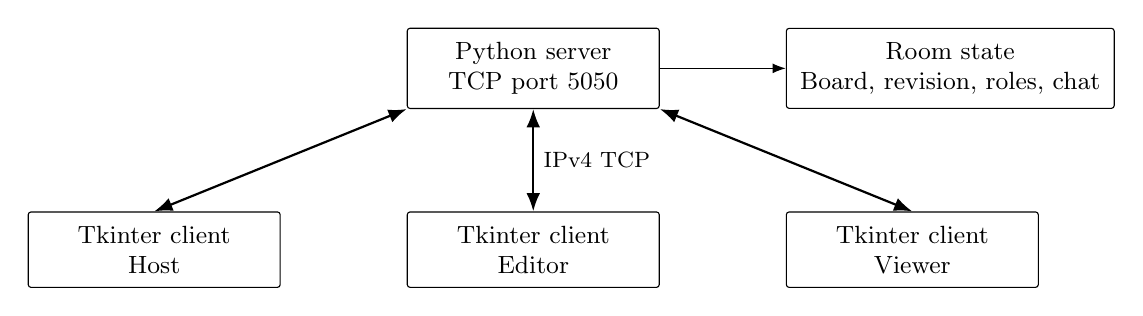
\begin{tikzpicture}
  \node[actor, minimum width=32mm] (server) {Python server\\TCP port 5050};
  \node[actor, minimum width=41mm, right=16mm of server] (state) {Room state\\Board, revision, roles, chat};
  \node[actor, minimum width=32mm, below=13mm of server] (editor) {Tkinter client\\Editor};
  \node[actor, minimum width=32mm, left=16mm of editor] (host) {Tkinter client\\Host};
  \node[actor, minimum width=32mm, right=16mm of editor] (viewer) {Tkinter client\\Viewer};
  \draw[wire] (host.north) -- (server.south west);
  \draw[wire] (editor.north) -- node[right,font=\footnotesize]{IPv4 TCP} (server.south);
  \draw[wire] (viewer.north) -- (server.south east);
  \draw[msg] (server) -- (state);
\end{tikzpicture}
\captionof{figure}{Each client has its own IPv4 TCP connection. The room state is maintained inside the server process.}
\label{fig:architecture}
\end{center}

\textbf{Server and sockets.}
\code{server.py} binds an IPv4 listening socket, accepts connections and starts a reader for each accepted socket. A separate writer drains that peer's outgoing queue. \code{client.py} handles drawing, chat, presence and reconnection. The workers use queues to communicate with the Tk event loop. \code{protocol.py} supplies the frame encoder, reader and shared limits.

\textbf{Why a central server and native GUI?}
One server can assign a common order and check permissions at the point where state changes. A peer-to-peer design would need a separate agreement mechanism for concurrent edits. The server is a single point of failure, so the host can save the board to a file. Tkinter provides direct canvas input and works offline with Python's standard library and Tk. Its widgets run on one event loop, so network I/O takes place on background threads.

\subsection{Room access and chat}

Two distinct eight-character codes grant editor or viewer access. A room creator is the host, and only the host can save, clear or restore. A viewer can chat and point. The server validates commands against the peer's role, associates edits with its username and checks payload bounds. Named, color-coded cursors distinguish participants. Chat is displayed in broadcast order with usernames and server-generated UTC timestamps converted to local time. Codes and resume tokens travel in plaintext TCP, so this access model assumes a trusted LAN.

\clearpage
\section{Application-level protocol}

TCP supplies an ordered, reliable byte stream within each connection~\cite{tcp}. Using UDP would move delivery, reordering and retransmission decisions into the application. With TCP, a lost segment can delay later bytes on that connection. The whiteboard sends small edit messages and uses an independent socket and writer queue for every peer.

The application frames each UTF-8 JSON object~\cite{json} with a four-byte unsigned big-endian body length. The header excludes its own four bytes. The receiver reads the exact length of the header and body, including when a frame arrives in pieces or when one write carries several frames. Bodies must be between one byte and 4 MiB and contain a string \code{type}. JSON keeps points, text and nested board snapshots easy to inspect. A dedicated binary schema would be smaller but would add encoding work to this project.

\command{00 00 00 0F\quad\{"type":"sync"\}}
The left side shows the prefix in hexadecimal. The right side is the literal 15-byte body requesting a snapshot.

\begin{center}
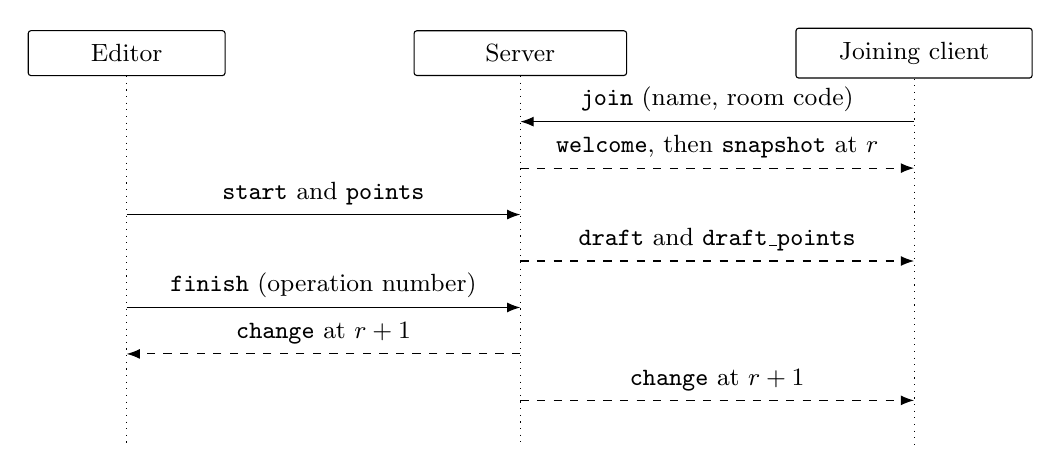
\begin{tikzpicture}[font=\small]
  \node[actor,minimum width=25mm] (e) at (0,0) {Editor};
  \node[actor,minimum width=27mm] (s) at (5,0) {Server};
  \node[actor,minimum width=30mm] (j) at (10,0) {Joining client};
  \foreach \lane in {e,s,j}
    \draw[dotted] (\lane.south) -- ++(0,-4.67);
  \draw[msg] (10,-.87) -- node[above]{\code{join} (name, room code)} (5,-.87);
  \draw[reply] (5,-1.46) -- node[above]{\code{welcome}, then \code{snapshot} at $r$} (10,-1.46);
  \draw[msg] (0,-2.05) -- node[above]{\code{start} and \code{points}} (5,-2.05);
  \draw[reply] (5,-2.64) -- node[above]{\code{draft} and \code{draft\_points}} (10,-2.64);
  \draw[msg] (0,-3.23) -- node[above]{\code{finish} (operation number)} (5,-3.23);
  \draw[reply] (5,-3.82) -- node[above]{\code{change} at $r+1$} (0,-3.82);
  \draw[reply] (5,-4.41) -- node[above]{\code{change} at $r+1$} (10,-4.41);
\end{tikzpicture}
\captionof{figure}{Join and drawing sequence. Only the joining client's draft updates are drawn. Draft updates also reach the editor, and the draft ends before the commit.}
\label{fig:sequence}
\end{center}

\small
\begin{tabularx}{\linewidth}{@{}P{36mm}Y@{}}
\toprule
\textbf{Message family} & \textbf{Payload and result}\\
\midrule
\code{create}, \code{join} & Username and room title or join code. A reconnect includes a resume token. The server sends \code{welcome} and then \code{snapshot}.\\
\code{start}, \code{points}, \code{finish}, \code{cancel} & Initial pen point and style, batches of up to 64 points, commit, or cancel.\\
\code{add}, \code{erase}, \code{undo}, \code{redo} & Add an item, target its ID, or move an action between user stacks. A \code{change} carries \code{rev}, \code{id} and the visible item or JSON \code{null}.\\
\code{save}, \code{clear}, \code{restore} & Host commands. Save returns \code{saved} with the versioned board. Clear and restore broadcast a \code{snapshot}.\\
\code{chat}, \code{presence}, \code{cursor} & Chat carries text and gains server-assigned sender and time. Presence carries the roster and notice. Cursor messages carry a participant ID and logical point in broadcasts. \code{cursor\_end} hides the pointer.\\
\code{sync}, \code{snapshot}, \code{heartbeat}, \code{error} & State request, state response, idle traffic, and rejected-command feedback.\\
\bottomrule
\end{tabularx}
\normalsize

{\small
\renewcommand{\refname}{Protocol references}
\begin{thebibliography}{9}
\setlength{\itemsep}{0pt}
\bibitem{tcp} W. Eddy (ed.), \href{https://www.rfc-editor.org/rfc/rfc9293}{\emph{Transmission Control Protocol (TCP)}}, RFC 9293, 2022.
\bibitem{json} T. Bray (ed.), \href{https://www.rfc-editor.org/rfc/rfc8259}{\emph{The JavaScript Object Notation (JSON) Data Interchange Format}}, RFC 8259, 2017.
\end{thebibliography}
}

\clearpage
\section{Synchronization and state management}

\subsection{Ordering and performance}

Peer readers can accept input concurrently. Within a room, a lock serializes command handling, state changes and queue insertion. Committed changes receive increasing room revisions. The server queues each broadcast in the same order for every peer, including the originator. Because writers perform socket I/O outside the room lock, a blocked socket does not block edits for the other peers. A full output queue disconnects its peer. A thread pair per connection keeps the classroom-scale code simple and consumes more resources as the number of connections grows.

A join queues \code{welcome} and a \code{snapshot} while holding the room lock. The snapshot contains the revision, visible items, active drafts, roster and up to 100 chat messages. Edits processed after the join follow the snapshot in that peer's queue. All clients therefore start from a known version and apply changes in the server's order.

The board uses a fixed $960\times600$ coordinate space. Each window scales that space to fit its canvas. Local pen movement is drawn immediately. The client batches pen points and sends changed cursor coordinates on a 33 ms timer. Peers see incremental drafts, and a commit carries one item. \code{TCP\_NODELAY} allows small writes to be sent without waiting for the Nagle algorithm. Point batches reduce traffic at the cost of a short wait before a remote preview can be shown. Full snapshots are reserved for initialization, recovery and board replacement.

\subsection{Concurrent undo, save and restore}

The server stores objects rather than pixels. An item includes an ID, tool kind, color, width, points and author, with text for sticky notes. Items are displayed in ID order to preserve stacking. An erasure hides a whole item by ID. A stroke is one undoable action when it is committed at release. Shapes, notes and erasures each record one action. Each participant has separate undo and redo stacks.

If A adds a rectangle and B erases it, A can undo and redo the addition while B's erasure remains active. The rectangle stays hidden until B undoes the erasure. This follows directly from the visibility rule. The insertion must be active and there must be no active erasures for that item. Per-user undo preserves other users' work and can leave the drawing visually unchanged when another action still hides an item.

Save writes visible committed items in a versioned JSON file on the host's machine. The client writes a temporary file beside the destination and then replaces the destination. Restore validates the full board before replacing room state. Restore and clear discard drafts and undo history and send a new snapshot. This retains a portable drawing after a restart while live rooms, chat and histories stay in memory.

\subsection{Duplicate detection and connection recovery}

Numbered edits and chat carry an increasing \code{op} per participant. The server ignores numbers at or below the last number it has seen for that participant. A client drops old revisions and requests \code{sync} when an incremental revision skips an expected value. It installs the next full snapshot before applying further increments.

Idle writers send a heartbeat after four seconds. Readers allow 14 seconds for a frame plus up to one polling interval. EOF or timeout removes the peer and cancels its unfinished draft. The client retries after one second and doubles the wait up to eight seconds. Its token resumes the original role, action stacks and operation counter. A new snapshot catches it up without replaying uncertain edits.

\clearpage
\section{User guide}

\textbf{Start the server.}
Connect the computers to the same LAN. Find the host's IPv4 address with \code{ipconfig} on Windows or \code{ip -4 addr} on Linux. Permit inbound TCP on the host's private network if prompted. For the source version, install Python 3.11 or later with Tk and check it with \code{python -m tkinter}. Some Linux distributions package Tk separately. Extract \code{source-code.zip} and run:

\command{python server.py --bind 0.0.0.0 --port 5050}

\textbf{Open each client.} Run the following on each participant's machine. On Linux, use \code{python3} if needed.

\command{python client.py}

\textbf{Create or join a room.} Enter the server's IPv4 address, port and a username. Use \code{127.0.0.1} when the client and server run on the same machine. The host enters a room name and selects \textbf{Create room}. Other users enter the editor or viewer code and select \textbf{Join room}.

\textbf{Collaborate.} Choose a color and width. Drag with Pen, Line, Arrow or Rectangle, or click with Note to enter an annotation. Click a committed object with Eraser to remove it. Undo and Redo work on your own actions. The participant list shows roles and the chat panel shows timestamped messages.

\textbf{Save and recover.} Use \textbf{Save board} to write a JSON file and \textbf{Restore board} to load it. \textbf{Clear board} asks for confirmation. Leave a disconnected client open so it can reconnect. If the server restarted, create a new room and restore a saved board.

\textbf{Windows standalone build.} From PowerShell in the executable directory on Windows x64, run:

\command{.\textbackslash{}WhiteboardServer.exe --bind 0.0.0.0 --port 5050}

Then open \code{WhiteboardClient.exe}. The binaries bundle their runtime. Linux source use still needs a test. Each target OS requires its own standalone build.

\begin{center}
  \screen{.86\linewidth}{02-shared-drawing}
  \captionof{figure}{The shared board in the running application. The toolbar, active pen strokes, participant list, room chat and host controls are visible. The README links the same capture.}
  \label{fig:client}
\end{center}

\clearpage
\section{Verification and requirement coverage}

Three Windows loopback clients exercised the user workflows below. In a separate socket test, two concurrent senders submitted 40 edits and all three peers received the same revisions in order. For 50 small commits, sender submission to remote socket receipt measured \textbf{0.12 ms median} and \textbf{0.22 ms p95}. Tk rendering and physical LAN latency are outside this measurement. The standalone server accepted a framed create request and returned a snapshot. The standalone client opened its lobby.

\small
\begin{tabularx}{\linewidth}{@{}P{36mm}Y@{}}
\toprule
\textbf{Course requirement} & \textbf{Implementation and checked behavior}\\
\midrule
Drawing and shared canvas & Freehand, colors, eraser, annotations and shape tools. Three clients converged on the same drawing. Host save, clear and restore updated the room as expected.\\
Rooms and participants & IPv4 and room-code setup, named pointers and join/leave notices. A late viewer received the existing board and chat, and an unauthorized command was rejected.\\
Sockets and event handling & Checked split and combined frames, concurrent broadcasts, duplicate suppression and idle timeout. A client test verified that a revision gap triggers a sync request.\\
Group chat & Room messages appeared in broadcast order with names and timestamps. Late and returning clients received recent chat.\\
State and recovery & Verified snapshots, disconnect/reconnect, removal of an unfinished draft and per-user undo and redo. An invalid restore left the board unchanged.\\
\bottomrule
\end{tabularx}
\normalsize

\begin{center}
  \screen{.44\linewidth}{03-late-join-viewer}\qquad
  \screen{.44\linewidth}{12-reconnected}
  \captionof{figure}{Late join (left) and recovery after reconnect (right). Each client displays the shared canvas and recent chat.}
\end{center}

\section{Team contributions}

\small
\begin{tabularx}{\linewidth}{@{}P{24mm}P{22mm}Y@{}}
\toprule
\textbf{Member} & \textbf{Roll number} & \textbf{Contribution}\\
\midrule
L. Guna & \textbf{cs24b2043} & TCP framing, socket lifecycle, concurrency and ordered broadcasts.\\
B. Rakesh & \textbf{cs24b2039} & Board state, per-user undo and redo, snapshots, persistence and reconnection.\\
L. Bhupesh & \textbf{cs24b2029} & Room creation and joining, presence, access control and chat.\\
R. Suhaas & \textbf{cs24b2040} & Tkinter workspace, canvas rendering, drawing tools and point batching.\\
\bottomrule
\end{tabularx}

\end{document}
